\chapter{Sejarah Lingkungan}
\section{Sejarah Lingkungan St. Petrus}
\small
Lingkungan Santa Theresia Kanak-kanak Yesus adalah lingkungan baru di Stasi Bunda Maria Maguwo. Lingkungan ini merupakan hasil pemekaran dari lingkungan St. Petrus yang dirasa sudah terlalu banyak anggotanya. Lingkungan St. Petrus dimekarkan menjadi lingkungan St. Petrus, lingkungan St. Monika, dan lingkungan St. Theresia.

Dengan demikian sejarah lingkungan St. Theresia tidak bisa lepas dari sejarah lingkungan St. Petrus. 
Pada awalnya, yaitu tahun 1984, bernama Kring Santo
Petrus yang meliputi dusun Nanggulan, Kopenrejo, Gondangan, Setan,
Dewan, Kalongan, dan Kembang. Kepengurusan periode awal ini diketuai
oleh Ig. Mulyono yang diberkati oleh Rm Y. Suyadi, Pr, romo Paroki
Kalasan saat itu. Kepengurusan ini berakhir pada tahun 1987.

Periode berikutnya 1987-1990 Kring St Petrus memiliki umat sebanyak 159
warga dalam 53 keluarga dan sebagai ketua kring adalah Th Sukamto. Pada
tahun 1990 status kring berubah menjadi lingkungan bersamaan dengan
perubahan Wilayah Maguwo menjadi Stasi Maguwo. Pada penyerahan
kepengurusan dari periode sebelumnya kepada H. Siswanto sebagai ketua
lingkungan periode 1990-1993, jumlah umat lingkungan St Petrus sudah
berkembang menjadi 71 keluarga yang terdiri atas 213 warga. Mengingat
wilayah St Petrus yang luas maka disepakati untuk dilakukan pemekaran
menjadi 2 lingkungan yaitu St Petrus dan St Paulus. Lingkungan St
Petrus meliputi Kembang, Nanggulan, Gondangan, Tajem, Setan, Karang
Nongko, Sopalan, Pugeran dan Sanggrahan. Lingkungan Paulus meliputi
Rejoinangun, Dewan, Kalongan, dan Corongan.

Periode berikutnya 1993-1995 umat lingkungan mencapai 58 keluarga
terdiri atas 223 warga dengan ketua Thomas Sukijo. Periode 1996-2001
ketua lingkungan dijabat oleh Valentinus Sukiyanto dengan umat sejumlah
256 warga dalam 69 keluarga. Saat ketua dijabat oleh Yoseph Samin
(2002-2004) umat berkembang menjadi 76 keluarga dengan 270 warga.

Wilayah Lingkungan St Petrus masih dirasa terlalu luas maka pada tahun
2006 saat kepengurusan FX Radjijo (2005-2007) dilakukan pemekaran lagi
menjadi 2 lingkungan yaitu St Petrus dan St Fransiskus Asisi.
Lingkungan St. Petrus meliputi Kembang, Nanggulan, Sanggrahan, Maguwo,
Karangnongko, Pugeran dan Sombomerten. 

Periode transisi 2006-2007 Lingkungan St Petrus diketuai oleh Y.Z.
Budiman S dengan umat sebanyak 162 orang dalam 48 keluarga. 

Periode 2008 -- 2010 Lingkungan St Petrus mempunyai umat sebanyak 187
orang dalam 63 keluarga dan diketuai oleh V. Agung Danan Jaya.

Dalam  periode kepengurusan 2011 -- 2013 Lingkungan St. Petrus kembali
dipimpin oleh Y.Z. Budiman Susanto, dengan jumlah umat sebanyak 193
jiwa dalam 62 keluarga. Pada tahun 2013, jumlah umat bertambah menjadi
199 jiwa dalam 63 keluarga.
\normalsize

\section{Lingkungan St. Theresia Kanak-kanak Yesus}
\begin{floatingfigure}[l]{2cm}
\begin{center}
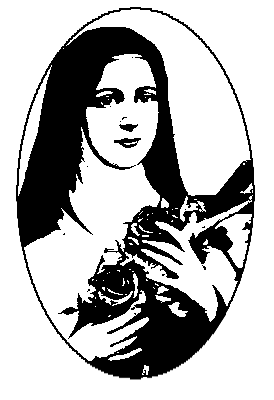
\includegraphics[scale=1]{theresia-logo.png}
\end{center}
\end{floatingfigure}
Pada akhir tahun 2013 yaitu pada bulan September, semua lingkungan di Stasi Maguwo 
diharapkan melakukan pemilihan pengurus baru. Sesuai dengan mekanisme pemilihan dari paroki, 
maka dilakukanlah pemilihan pengurus baru yang diketuai oleh Andreas Keso Muda.
Pemilihan berhasil memilih Anton Supriyana sebagai ketua baru. Beliau ini adalah warga baru namun stok lama. Beliau sudah lama berkecimpung di dewan paroki Pringwulung, tempat tinggal beliau sebelumnya.

Berdasar diskusi dengan beberapa umat akhirnya terbentuklah susunan pengurus baru lingkungan St. Petrus dan sempat disosialisasikan pada ibadat lingkungan di rumah Agung Danan Jaya pada tanggal 12 September 2013. Namun pada tanggal 13 September 2013 setelah ada imbauan dari paroki dan stasi untuk pemekaran lingkungan, maka muncullah ide pemekaran lingkungan. Dari diskusi beberapa umat disimpulkan bahwa jika ingin mekar, harus dilakukan saat itu juga. Maka dengan gerak cepat beberapa umat mencoba mematangkan ide tersebut dan kemudian dilontarkan pada pertemuan calon pengurus baru lingkungan St. Petrus pada tanggal 15 September 2013 di rumah Bapak Anton. Ternyata ide tersebut didukung sepenuhnya oleh calon ketua lingkungan dan peserta pertemuan. Tindakan selanjutnya adalah pembentukan pengurus di masing-masing lingkungan hasil pemekaran, yaitu 3 lingkungan. 

Lingkungan Petrus 1 meliputi Kembang, Nanggulan, dan Tobong. Petrus 2 meliputi Maguwo, Sanggrahan, dan Karangnongko. Petrus 3 meliputi Pugeran dan Sombomerten. Disepakati juga bahwa nama St. Petrus tetap digunakan untuk Petrus 1 karena awal lingkungan St. Petrus ada di Nanggulan. Nama pelindung untuk Petrus 2 dan Petrus 3 diserahkan kepada masing-masing lingkungan.

Pemilihan pengurus untuk lingkungan Petrus 3 dilaksanakan pada tanggal 16 September 2013 bertempat di rumah Bapak Supriyadi. Secara mufakat terpilih Bapak Anton sebagai ketua lingkungan dan tersusun dengan cepat pengurus-pengurus lainnya. Setelah melalui mekanisme penggalian informasi dari umat melalui sms ditetapkan bahwa nama pelindung lingkungan Petrus 3 adalah \textbf{Santa Theresia dari Kanak-kanak Yesus} atau nama singkatnya \textbf{Santa Theresia}.

Untuk lingkungan Petrus 1 terpilih Bapak Hananto sebagai ketua melalui pertemuan pada tanggal 18 September 2013 di rumah Bapak Hananto. Sedang untuk Petrus 2 melalui pertemuan pada tanggal 20 September 2013 di rumah Bapak Yos terpilih Bapak Budi sebagai ketua. Akhirnya umat lingkungan Petrus 2 sepakat menggunakan nama pelindung Santa Monica.

Lingkungan St. Theresia mencakup 25 keluarga dengan 80 umat dengan perincian 34 laki-laki dan 46 perempuan. Namun demikian ada beberapa mahasiswa yang terlibat aktif dalam kegiatan-kegiatan lingkungan dan tidak tercatat dengan pasti karena mobilitasnya yang tinggi.

\section{Riwayat St. Theresia Kanak-kanak Yesus}
Santa Theresia dari kanak-kanak Yesus dilahirkan di Alemon Perancis pada tgl 2 Januari 1873 dengan nama Maria Francoise Therese Martin. Ia berasal dari sebuah keluarga Katolik yang saleh, pasangan suami isteri Louis Martin dan Azelie Guerin. Ibunya meninggal waktu Theresia masih anak-anak. Sepeninggal ibu Theresia sangat terguncang sehingga Pauline kakaknya terpaksa menggantikan peran ibunya untuk merawat dan memperhatikan perkembangan Theresia.

\begin{floatingfigure}[l]{2.75cm}
\begin{center}
\includegraphics[scale=0.5]{theresia-1.jpg}
\end{center}
\end{floatingfigure}
Theresia sangat disayang oleh ayahnya dan mendapat berbagai julukan seperti "Theresia kecil" atau "Ratu Kecil" dsb. Tahun 1881 sampai 1885 Theresia bersekolah di sekolah suster-suster Benedictin, ia tumbuh menjadi seorang gadis kecil yang sangat perasa dan cepat menangis sehingga kurang akrab dengan teman-teman sekolahnya. Sifat perasanya semakin menjadi-jadi ketika Pauline kakak perempuannya masuk biara Carmel di Lisieux tahun 1882. Theresia jatuh sakit karena keberangkatan kakaknya itu, namun ia disembuhkan secara ajaib saat kakak-kakaknya berlutut dan berdoa disamping tempat tidur untuk kesembuhannya, penyakitnya hilang seketika meskipun sifat perasanya masih ada. Sifat perasa itu baru hilang setelah dinasihati oleh ayahnya pada perayaan Natal 1886, semenjak itu ia sadar akan sifat buruknya yang manja dan mudah tersinggung itu. Ia sadar bahwa sifat yang kekanak-kanakan itu sudah tidak cocok lagi bagi seorang remaja puteri yang bercita-cita menjadi suster.

\begin{floatingfigure}[r]{3.75cm}
\begin{center}
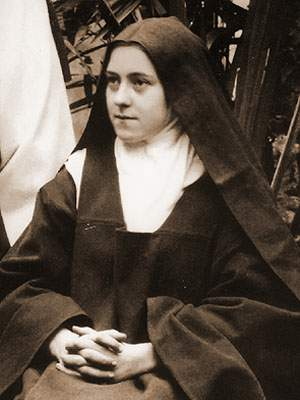
\includegraphics[scale=0.35]{theresia-2.jpg}
\end{center}
\end{floatingfigure}
Dalam autobiografinya, Theresia menyebutkan bahwa kesadaran ini mengawali kehidupannya yang baru, dimana Yesus telah menyembuhkannya dan menghilangkan sifat kepribadiannya yang buruk. Semenjak saat itu ia sadar bahwa dirinya dipenuhi oleh Roh Kudus, ia sadar bahwa ia harus mengabdikan seluruh hidupnya kepada Tuhan. Kerinduaanya untuk bersatu dengan kanak-kanak Yesus sangatlah besar dan oleh karena itulah dikemudian hari ia digelari "Santa Theresia dari Kanak-kanak Yesus". Kepada Yesus ia berjanji tidak akan pernah segan untuk melakukan apa saja yang dikehendaki Tuhan darinya. Betapa bahagia hati Theresia ketika pada umur 12 tahun ia boleh menyambut komuni untuk pertama kalinya. Dihadapan sebuah salib ia berjanji: "Yesus di kayu salib yang haus, saya akan memberikan air kepadaMu. Saya bersedia menderita sedapat mungkin agar banyak orang berdosa yang bertobat. Kerinduan Theresia yang begitu besar kepada Yesus mendesak ia untuk menjalani khusus sebagai biarawati mengikuti jejak ke 4 saudaranya yang lebih dahulu menjadi biarawati, namun ia belum bisa diterima di biara karena umurnya baru 14 tahun.

Pada umur 15 tahun saat berziarah ke Roma bersama ayahnya, Theresia dengan meminta izin khusus dari Bapa Suci agar ia diperkenankan menjadi biarawati. Permintaannya dikabulkan dan ia masuk diterima di lingkungan biara Carmelit di Lisieux Perancis.

Sembilan tahun lamanya ia hidup sebagai suster biasa, dan sebagaimana biasanya seorang suster muda, ia setiap hari melaksanakan tugas dan doa harian, harus mengatasi perasaan marah, tersinggung, iri hati, memerangi kebosanan dan berbagai ragam godaan lahir maupun batin. Untuk mencapai kesempurnaan hidup ia memilih "Jalan Sedehana" berdasarkan ajaran kitab suci yaitu hidup selaku anak kecil, penuh cinta dan iman akan kepercayaan Allah serta penyerahan diri yang total dengan penuh perasaan gembira. Demi cita-cita itu ia melakukan hal-hal kecil dan kewajiban sehari-hari di biara dengan penuh tanggung jawab karena cinta kasihnya yang besar kepada Allah Bapa di surga.

Ia sedih sekali melihat banyak orang menyakiti hati Yesus dengan berbuat dosa dan tidak mau bertobat. Untuk mempertobatkan orang-orang berdosa itu, ia mempersembahkan dirinya sebagai korban pepulih dosa-dosa. Ia rajin berdoa dan melakukan tapa bagi semua orang berdosa. Ia juga berdoa bagi para missionaris dan kemajuan kerajaan Allah di seluruh dunia.

Theresia akhirnya menderita sakit paru-paru yang sangat parah. Selama 2 tahun ia menanggung beban penderitaan itu dengan gembira. Penyakit ini kemudian merenggut nyawanya pada tanggal 30 September 1897 di biara Lisieux. Sebelum menghembuskan nafasnya ia berjanji untuk menurunkan hujan mawar ke dunia. Janji ini terpenuhi dengan banyaknya karunia Allah yang diberikan kepada semua orang yang berdoa dengan perantaranya. Theresia meninggal dalam usia yang sangat muda 24 tahun. Pada tahun 1925 ia ditetapkan sebagai "Santa" oleh Paus Pius XI (1922-1939) dan diangkat menjadi Santa pelindung negara Perancis oleh Paus Pius XII (1939-1958)

\subsubsection*{Setelah Theresia Wafat}

Setelah wafat, Theresia menjadi terkenal karena buku yang ditulisnya "Kisah Suatu Jiwa," yang diterbitkan satu tahun setelah wafatnya (di Indonesia diterjemahkan dengan judul: 'Aku Percaya akan Cinta Kasih Allah'). Theresia dikanonisasi pada tahun 1925 oleh Paus Pius X. Ia dikenal dengan sebutan Santa Theresia dari Kanak-kanak Yesus atau Santa Theresia si Bunga Kecil. St. Theresia bersama-sama dengan St. Jeanne d'Arc diberi gelar Pelindung Perancis. Selain itu St. Theresia bersama-sama dengan St. Fransiskus Xaverius diberi gelar Pelindung Misionaris.  Pada tanggal 19 Oktober 1997, Theresia juga menjadi wanita ke-3 yang diberi gelar Doktor Gereja. Kita dapat mohon bantuannya mengenai apa saja. Ia pernah berjanji  akan melimpahi kita dengan bunga-bunga mawar dari surga dan memang, sejak kematiannya banyak mukjizat yang terjadi berkat bantuan doanya. Pestanya diraya-kan setiap tanggal 1 Oktober.

\subsection*{Rahasia Theresia: Jalan Kecil, Jalan Kanak-Kanak Rohani}

\begin{floatingfigure}[l]{2.75cm}
\begin{center}
\includegraphics[scale=0.275]{theresia-3.jpg}
\end{center}
\end{floatingfigure}
Theresia seorang gadis yang sederhana dengan `jalan kecilnya' yang istimewa.  Ia menunjukkan bahwa \textbf{kekudusan dapat dicapai oleh siapa saja betapa pun rendah, hina dan biasanya orang itu}. Caranya ialah dengan melaksanakan pekerjaan-pekerjaan kecil dan tugas sehari-hari dengan penuh cinta kasih murni kepada Tuhan. Kamu pun dapat menjadi kudus dengan cara-cara sederhana seperti yang dilakukan oleh St. Theresia dengan jalan kecilnya.

